\قسمت{بررسی تاثیر استفاده از انتگرال فازی در بهبود دانش جمعی}
همانطور که در بخش‌های قبلی دیدیم، استفاده از توابع $g(\cdot)$ مختلف در انتگرال فازی نتایج روش پیشنهادی موثر واقع شده‌اند و در نهایت با استفاده از تابع $\text{Const-One}$ که باعث می‌شود انتگرال فازی به یک عملگر بیشینه‌گیری تبدیل شود و بطور حریصانه در هر مرحله‌ی به اشتراک‌گذاری دانش، فقط دانش عاملی را به عنوان دانش جمعی خروجی الگوریتم در نظر بگیرد؛ در این بخش می‌خواهیم این موضوع را بررسی کنیم که تاثیر انتگرال فازی در بهبود دانش جمعی چگونه می‌باشد؟ به عنوان مثال آیا همیشه استفاده از انتگرال فازی در بهبود دانش جمعی موثر واقع است؟

در پاسخ به این سوالات، ما روش SEP را با این‌بار با استفاده از انتگرال فازی مورد آزمون قرار دادیم که همانطور که در شکل‌ \ref{fig:sep_maze_fci} مشاهده می‌کنیم وقتی در روش SEP بجای میانگین وزنی (روش پیشنهادی \مق{SEP}) از انتگرال فازی با توابع معرفی شده در الگوریتم‌های \ref{alg:g:max} تا \ref{alg:g:k-mean} استفاده کنیم برعکس نتایج بدست آمده خروجی انتگرال فازی کیفیت و سرعت یادگیری را بهبود نبخشید -- گرچه ممکن است در صورت تعریف توابع $g(\cdot)$ دیگر نتایج بهتری تولید کند؛ ولی در صورتی که از الگوریتم \ref{alg:g:const-one} استفاده کنیم بهترین نتیجه‌ی ممکن را می‌گیریم.

\begin{figure}
\centering
\caption{تاثیر استفاده از انتگرال فازی در روش SEP بروی کیفیت و سرعت یادگیری در محیط پلکان مارپیچ}\label{fig:sep_maze_fci}
\begin{tabular}{*1c}
\subf{\includegraphics[width=.8\textwidth]{boltzmann/pref/sep/env/maze/fci-check.png}}
     {الف - استفاده از انتگرال فازی در روش SEP در محیط پلکان مارپیچ}
\\
\subf{\includegraphics[width=.8\textwidth]{boltzmann/pref/sep/env/prey/fci-check.png}}
{ب - استفاده از انتگرال فازی در روش SEP در محیط صید و صیاد}
\end{tabular}
\end{figure}

در مورد روش MCE نیز تاثیر استفاده از انتگرال فازی را نیز مورد بررسی قرار دادیم که در شکل \ref{fig:mce_maze_fci} نتایج آمده است. همانطور که مشاهده می‌شود انتگرال فازی در روش MCE با توابع $g(\cdot)$ معرفی شده در این پژوهش (یعنی الگوریتم‌های \ref{alg:g:const-one} تا \ref{alg:g:k-mean}) باعث بهبود نتایج شده است. این بهبود در محیط پلکان مارپیچ به صورت بهبود در سرعت یادگیری و در محیط صید و صیاد در سرعت و کیفیت یادگیری مشاهده می‌شود. همانطور که در بخش‌ها قبلی نیز آورده شده است، انتگرال فازی روشی جامع‌تر از میانگین‌گیری وزن‌دار می‌باشد و در همانطور که از نتایج آزمایش‌های این فصل می‌توان برداشت کرد با انتخاب و معرفی مناسب تابع $g(\cdot)$ انتگرال فازی می‌تواند نتایج بهتری نسبت به روش میانگین‌گیری وزندار تولید نماید -- این نتیجه‌گیری را می‌توان در بهبود نتایج توسط کلیه‌ی توابع $g(\cdot)$ معرفی شده در این پژوهش بروی روش پیشنهادی و MCE و همچنین تابع \ref{alg:g:const-one} بروی روش SEP مشاهده کرد. همچنین با توجه به نتایج حاصل در شکل \ref{fig:mce_maze_fci} باید به این نکته توجه کرد که انتخاب حریصانه‌ی دانش عامل‌ها به عنوان دانش جمعی (یعنی انتخاب توابع \مق{Const-One} -- الگوریتم \ref{alg:g:const-one} به عنوان تابع $g(\cdot)$) همیشه موثر نمی‌باشد.

\begin{figure}
\centering
\caption{تاثیر استفاده از انتگرال فازی در روش MCE بروی کیفیت و سرعت یادگیری در محیط پلکان مارپیچ}\label{fig:mce_maze_fci}
\begin{tabular}{*1c}
\subf{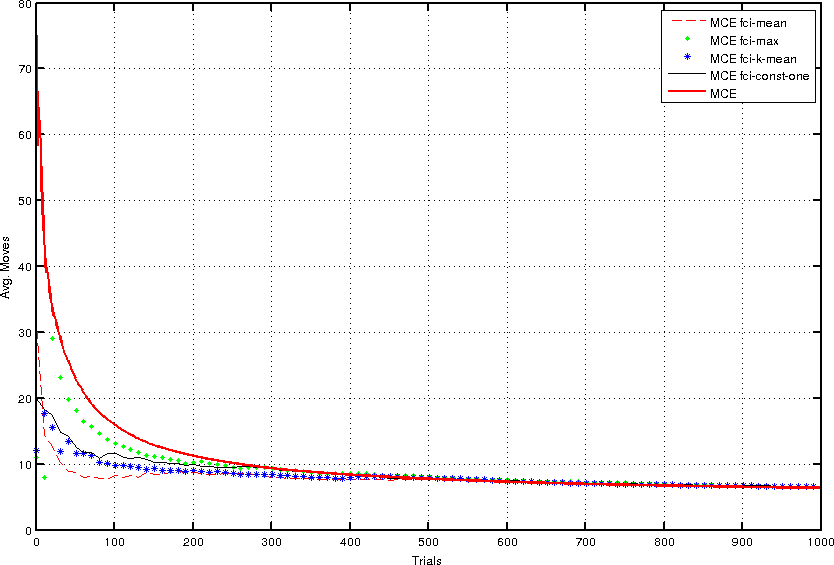
\includegraphics[width=.8\textwidth]{boltzmann/pref/mce/env/maze/mce-fci-maze.png}}
     {الف - استفاده از انتگرال فازی در روش MCE در محیط پلکان مارپیچ}
\\
\subf{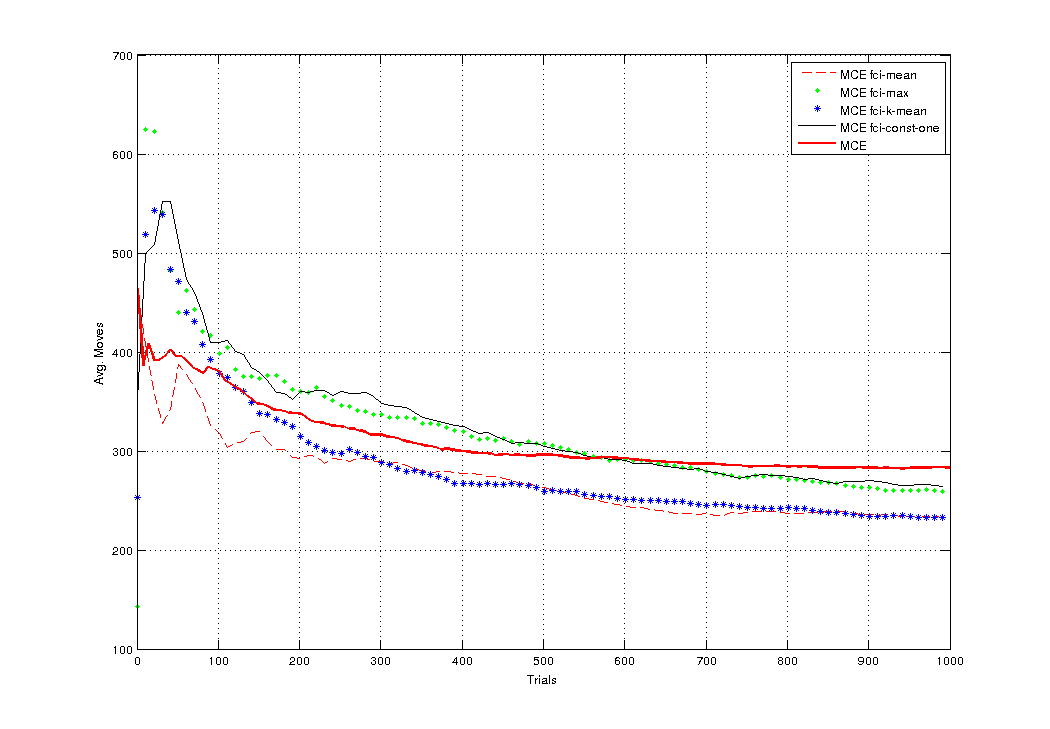
\includegraphics[width=.8\textwidth]{boltzmann/pref/mce/env/prey/mce-fci-prey.png}}
{ب - استفاده از انتگرال فازی در روش MCE در محیط صید و صیاد}
\end{tabular}
\end{figure}